\documentclass[12pt]{article}
\usepackage{hyperref}
\usepackage{amsmath}
\usepackage{amsfonts}
\usepackage{amssymb}
\usepackage{graphicx}
\usepackage{caption}
\usepackage{enumerate}

\title{\Huge\textbf{CS215 Assignment 2}}
\author{\Large\textbf{ Group Members :} \\ \\ 
    \large B.Abhinav  23B1018 \\ \\ 
    \large G.Abhiram  23B1084 \\ \\
    \large U.Sai Likhith 23B1058 
} 
\date{\today}
\counterwithin*{equation}{subsection}

\begin{document}



\pagenumbering{arabic}
\maketitle
\newpage

\tableofcontents
\newpage

%%%%%%%%%%%%%%%%%%%%%%%% Question 1 %%%%%%%%%%%%%%%%%%%%%%
\section{Mathemagic}
\subsection{Task A}
\textbf{Solution: } \newline
Lets derive the PGF for $X \sim \text{Ber}(p)$. PMF for Ber(p) is given by :
\[P(X=1) = p\]
\[P(X=0) = 1-p\]
G(z) for Bernoulli random variable is given by:

\[G_{Ber}\ =\ E(z^X)\ =\ \sum_{n=0}^{1}P[X\ =\ n]z^n \]

\begin{equation}
    G_{Ber}\ =\ (1-p)z^0+pz^1\ =\ 1-p+pz
\end{equation}

\subsection{Task B}
\textbf{Solution: } \newline
PMF of Bin(n, p) is given by: 
\[P(X=k)\ =\ \binom{n}{k}p^k(1-p)^{n-k}\]
G(z) for Binomial random variable is given by:

\[G_{Bin}\ =\ \sum_{k=0}^nP[X\ =\ k]z^k\]
\[G_{Bin}\ =\ \sum_{k=0}^n\binom{n}{k}(zp)^k(1-p)^{n-k}\]
Using Binomial Theorem :
\[G_{Bin}\ =\ (1-p+zp)^{n}\]
From $G_{Ber}$ in Task A:
\begin{equation}
    G_{Bin}\ =\ G_{Ber}(z)^n
\end{equation}

\subsection{Task C}
\textbf{Solution: } \newline
$X_1,X_2,X_3,\dots,X_k$ are independent non-negative-integer-valued random variables, each distributed with the same probability mass function P and have a common PGF G.
\[X\ =\ X_1+X_2+X_3+\dots+X_k\]
PGF of X is given by :
\[G_{\Sigma}\ =\ E(z^X)\ =\ E(z^{X_1+X_2+X_3+\dots+X_k})\]
\[G_{\Sigma}\ =\ E(z^{X_1}z^{X_2}z^{X_3}\dots z^{X_k})\]
Using the fact that when a, b are 2 independent random variables we have:
\begin{equation}
    E(f(a)g(b))\ =\ E(f(a))E(g(b))
\end{equation}
The proof is as follows:
\[E(f(a)g(b))\ =\ \sum_{a_i\in S(a)}^{}\sum_{b_j\in S(b)}^{}P_a[a=a_i]P_b[b=b_j]a_ib_j\]
As they are independent ie a,P(a) do not depend on b we get:
\[E(f(a)g(b))\ =\ \sum_{a_i\in S(a)}^{}P_a[a=a_i]a_i\sum_{b_j\in S(b)}^{}P_b[b=b_j]b_j\]
This proves the result.
As all $X_i$ are independent we have :

\[G_{\Sigma}\ =\ E(z^{X_1})E(z^{X_2})E(z^{X_3})\dots E(z^{X_k})\]
As all of them have common PGF G we get:
\begin{equation}
    G_{\Sigma}\ =\ G(z)^k
\end{equation}

\subsection{Task D}
\textbf{Solution: } \newline
PMF of Geo(p) is as follows:
\[P[X\ =\ n]\ =\ (1-p)^{n-1}p\]
where X = {1, 2, 3....} . PGF of Geo(p) is :
\[\sum_{n=1}^{\infty}P[X=n]z^n\ =\ \sum_{n=1}^{\infty}(1-p)^{n-1}pz^n\]
\[G_{Geo}\ =\ \frac{p}{1-p}\sum_{n=1}^{\infty}(z(1-p))^n\]
This summation only converges when:
\begin{equation}
    |z(1-p)|<1 \Rightarrow |z|<\frac{1}{|1-p|}
\end{equation}
Using the formula for sum of infinite GP:
\[G_{Geo}\ =\ \frac{p}{1-p}\times\frac{z(1-p)}{1-z(1-p)}\]
under the condition (5) Simplifies to:
\begin{equation}
    G_{Geo}\ =\ \frac{zp}{1-z+zp}
\end{equation}

\subsection{Task E}
\textbf{Solution: } \newline
Consider $X \sim \text{Bin}(n, p)$ and $Y \sim \text{NegBin}(n, p)$ .\\
Let us compute the PGF for Y using the result (4) from Task C. We know that NegBin(n, p) random variable can be written as sum of n independent Geo(p) random variables.
\[G_{Y}^{(n,p^{-1})}(z^{-1})\ =\ G_{Geo}^{p^{-1}}(z^{-1})^{n}\]
Using (6) with p and z replaced with $p^{-1}$ and $z^{-1}$ We ge :
\[G_{Y}^{(n,p^{-1})}(z^{-1})\ =\ \left(\frac{z^{-1}p^{-1}}{1-z^{-1}+z^{-1}p^{-1}}\right)^{n}\]
This simplifies to:
\[G_{Y}^{(n,p^{-1})}(z^{-1})\ =\ \left(\frac{1}{1-p+zp}\right)^{n}\]
Inverse on both sides and using (2):
\[\left(G_{Y}^{(n,p^{-1})}(z^{-1})\right)^{-1}\ =\ (1-p+zp)^n\ =\ G_{X}^{(n,p)}(z)\]
Replacing p with $p^{-1}$ and $z^{-1}$ we prove the result and inverting:
\begin{equation}
    G_{Y}^{(n,p)}(z)\ =\ \left(G_{X}^{(n,p^{-1})}(z^{-1})\right)^{-1}
\end{equation}

\subsection{Task F}
\textbf{Solution: } \newline
PMF of $Y \sim \text{NegBin}(n, p)$ is given by(for k = n, n+1, $\dots$):
\begin{equation}
    P[Y\ =\ k]\ =\ \binom{k-1}{n-1}p^n(1-p)^{k-n}
\end{equation}
The RHS of the equation (7) simplifies to:
\[(1-p^{-1}+z^{-1}p^{-1})^{-n}\ =\ \left(\frac{p^{n}z^{n}}{(1-z+pz)^n}\right)\]
The PGF of NegBin(n, p) by definition was:
\[G_Y^{(n,p)}\ =\ E(z^Y)\ =\ \sum_{k=n}^{\infty}\binom{k-1}{n-1}p^n(1-p)^{k-n}z^k\]
Equate both of them and use k = n + r on LHS:
\[\sum_{r=0}^{\infty}\binom{n+r-1}{n-1}p^n(1-p)^{r}z^{r+n}\ =\ \frac{p^{n}z^{n}}{(1-z+pz)^n}\]
Cancelling the common terms this simplifies to:
\[(1-z(1-p))^{-n}\ =\ \sum_{r=0}^{\infty}\binom{n+r-1}{n-1}(z(1-p))^{r}\]
We have proved in (5) that PGF for Y is only defined under $|z(1-p)<1$. \\
Substitute x = z(1-p) under $|x|<1$ to get:
\[(1-x)^{-n}\ =\ \sum_{r=0}^{\infty}\binom{n+r-1}{n-1}x^r \]
Using \[\binom{n}{r} = \binom{n}{n-r}\] and substituting x with -x we get:
\begin{equation}
    (1+x)^{-n}\ =\ \sum_{r=0}^{\infty}(-1)^{r}\binom{n+r-1}{r}x^r
\end{equation}
From the general definition of $\binom{n}{r}$ we have:
\[\binom{-n}{r}\ =\ \frac{(-n)(-n-1)(-n-2)....(-n-r+1)}{r!}\]
\[\binom{-n}{r}\ =\ (-1)^{r}\frac{(n+r-1)(n+r-2)...(n+1)(n)}{r!}\]
\[\binom{-n}{r}\ =\ (-1)^{r}\binom{n+r-1}{r}\]
Using this in (9) we get \\
For $n\in N$ and $|x|<1$ :
\begin{equation}
    (1+x)^{-n}\ =\ \sum_{r=0}^{\infty}(-1)^{r}\binom{n+r-1}{r}x^r\ =\ \sum_{r=0}^{\infty}\binom{-n}{r}x^r
\end{equation}
that is the Binomial Theorem for negative exponent.

\subsection{Task G}
\textbf{Solution: } \newline
We have for a random variable X with PGF G(z)
\[G(z)\ =\ \sum_{n=0}^{\infty}P[X=n]z^n\]
\[G'(z)\ =\ \sum_{n=0}^{\infty}nz^{n-1}P[X=n]\]
Substituting z = 1 we get:
\begin{equation}
    E(X)\ =\ \sum_{n=0}^{\infty}nP[X=n]\ =\ G'(1)
\end{equation}
Mean for Bern(p):
\[E_{Ber}\ =\ G'_{Ber}(1),\ G_{Ber}(z)=1-p+zp \Rightarrow G'_{Ber}(z)=p \]
Hence :
\begin{equation}
    E_{Ber}\ =\ p
\end{equation}
Mean for Bin(n, p)
\[G_{Bin}(z)\ =\ (1-p+zp)^n \Rightarrow G'_{Bin}(z)=np(1-p+zp)^{n-1} \Rightarrow G'_{Bin}(1)=np\]
Hence 
\begin{equation}
    E_{Bin}\ =\ np
\end{equation}
Mean for Geo(p)
\[G_{Geo}(z)\ =\ \frac{zp}{1-z+zp} \Rightarrow G'_{Geo}(z)=\frac{(1-z+zp)(p)-(zp)(p-1)}{(1-z+zp)^2}\]
\[G'_{Geo}(z)\ =\ \frac{p}{(1-z+zp)^2} \Rightarrow G'_{Geo}(1)=\frac{1}{p}\]
Hence
\begin{equation}
    E_{Geo}(z)\ =\ \frac{1}{p}
\end{equation}
Mean for NegBin(n, p)
\[G_{NegBin}(z)\ =\ G_{Geo}(z)^{n} \Rightarrow G'_{NegBin}(z)=nG_{Geo}(z)^{n-1}G'_{Geo}(z)\]
\[G'_{NegBin}(1)\ =\ \frac{n}{p}\]
Hence 
\[E_{NegBin} =\ \frac{n}{p}\]

%%%%%%%%%%%%%%%%%%%%%%%%%%%%%%%%%%%%%%%%%%%%%%%%%%%%%%%%%%%%%%

\section{Normal Sampling}
\subsection{Task A}
\textbf{Solution: } \newline
It suffices to prove that $f_{Y}(y)=1$,
Let us prove the following theorem first: \\
Given random variables $X$ and $Y$ with PDFs $f_X(x)$ and $f_Y(y)$, under an invertible transformation $Y = g(X)$, 
\[
f_Y(y) = \frac{f_X(g^{-1}(y))}{\left| g'(g^{-1}(y)) \right|}
\]
\textbf{Proof:} \\
Let $x_1, x_2, y_1, y_2 \in \mathbb{R}$ such that $y_1 = g(x_1)$ and $y_2 = g(x_2)$.
We have we have assuming g is non decreasing::
\[
P(x_1 \leq X \leq x_2) = P(y1 \leq Y \leq y2)
\]
since $g$ is invertible.
The probability of the event must be the same whether expressed in terms of $X$ or $Y$. This can be written as:
\[
\int_{x_1}^{x_2} f_X(x) \, dx = \int_{y_1}^{y_2} f_Y(y) \, dy
\]
Using the transformation $y = g(x)$, we know that:
\[
x=g^{-1}(y)\ and\ dx=(g^{-1})'(y)dy
\]
Thus, the integral becomes:
\[
\int_{y_1}^{y_2} f_Y(y) \, dy = \int_{y_1}^{y_2} f_X(g^{-1}(y))(g^{-1})'(y)dy
\]
As the above is true $\forall y1,y2 \in R$, The integrands must be equal.This can also be shown by treating them as functions and differentiating both integrals.(Second Fundamental Theorem of Calculus)
\[
f_Y(y) \ =\ f_X(g^{-1}(y)) \cdot (g^{-1})'(y)
\]
From calculus we have $(g^{-1})'(y)=\frac{1}{g'(g^{-1}(y))}$. It follows that:

\[
\boxed{f_Y(y) = \frac{f_X(g^{-1}(y))}{\left| g'(g^{-1}(y)) \right|}}
\]
The modulus is accounting for the case when g is non increasing as PDF's are always non negative.
Coming back to our question the invertible transformation $g$ is $F_{X}$ the CDF of X.
\[g(x)=\int_{-\infty}^{x}f_{X}(x)dx\  \Rightarrow\ g'(x)=f_{X}(x) \] 
Therefore here we have $g'(g^{-1}(y))=f_{X}(g^{-1}(y))$ and $g'\ge 0$ as CDF is non decreasing we have :
\[f_{Y}(y)=1\]
Therefore we proved that $Y$ is uniformly distributed in $[0,1]$.

\subsection{Task B}
From the theorem we have proved in Task A we can sample a standard normal distribution.
Let X be a standard normal disrtribution. We have
\[f_X(x) = \frac{1}{\sqrt{2\pi}} e^{-\frac{x^2}{2}}\]
Since $F_{X}'(x)=f(x) > 0\ \ ,F_{X}(x)$ is invertible.
We know that $Y=F_{X}(X)$ is a uniform distribution in [0,1] from Task A.\\
Our algorithm $\mathcal{A}$ invloves computing the inverse $G_{X}(Y)$ of $F_{X}(X)$ and then mapping the uniform distribution $Y$ using it.\\
Using this we can sample a standard normal distribution from a uniform distribution Y in [0,1].\\
This also implies that $\forall u \in R$ we have 
\[F_{\mathcal{A}}(u)=F_{X}(u)\ and\ f_{\mathcal{A}}(u)=f_{X}(u)\]

\subsection{Task C}
\textbf{Check the code in 2c.py}
\begin{minipage}{\linewidth}
    \begin{center}
        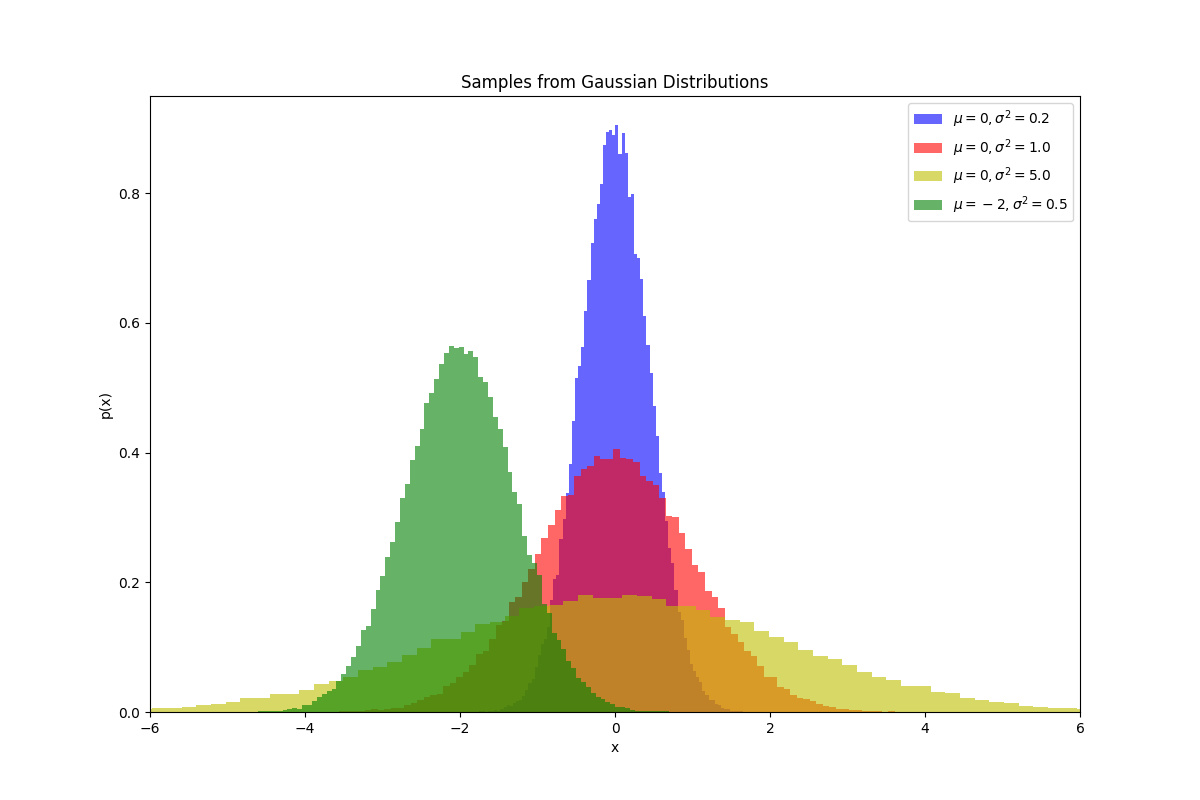
\includegraphics[width=0.5\textwidth]{images/2c.png}
        \captionof{figure}{The Bell curve}
    \end{center}
\end{minipage}

\subsection{Task D}
\textbf{Check the code in 2d.py} \\
The shape of the graph, which appears to be approximately bell-shaped for large depth(h), suggests that the distribution of the final positions of the balls is approximately normal.
\newline
This is because :
\begin{enumerate}
    \item The majority of the balls tend to fall in the middle pockets.
    \item The number of balls in each pocket decreases as you move away from the middle.
    \item The distribution is symmetric around the middle.
\end{enumerate}
\begin{minipage}{\linewidth}
    \begin{center}
        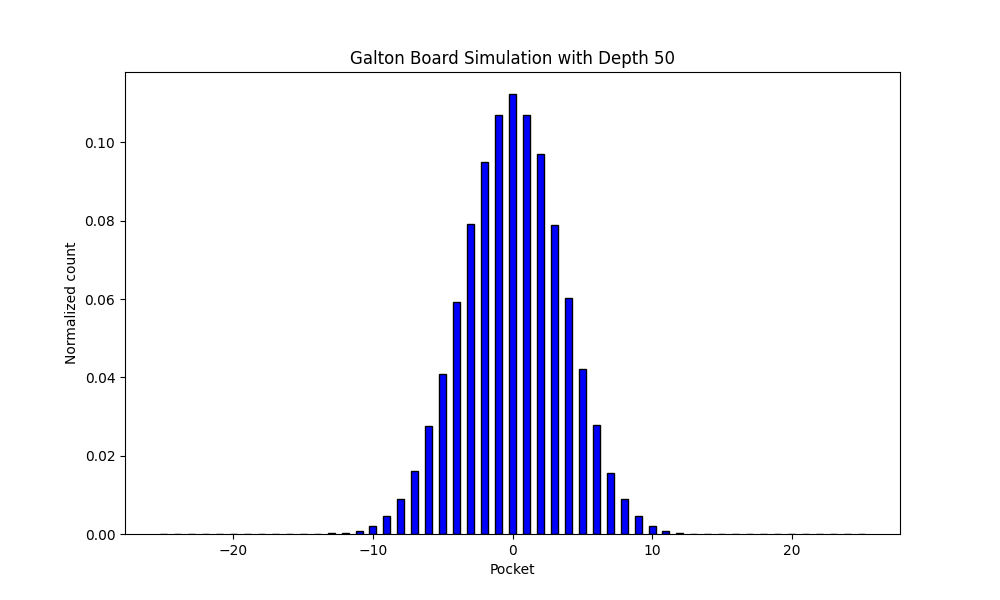
\includegraphics[width=0.5\textwidth]{images/2d2.png}
        \captionof{figure}{Plot for h = 50 and N = 100000}
    \end{center}
\end{minipage}
\begin{minipage}{\linewidth}
    \begin{center}
        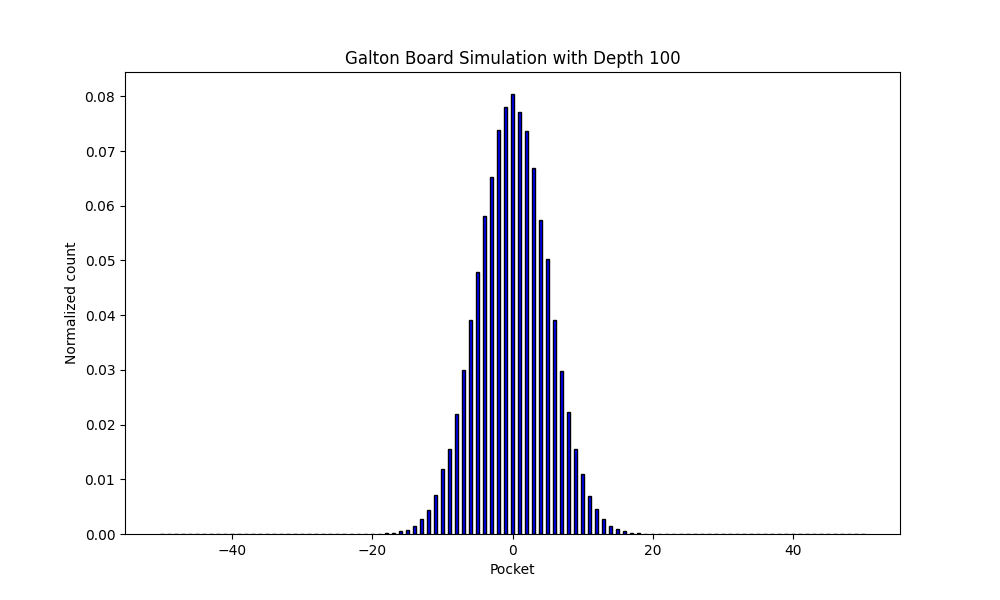
\includegraphics[width=0.5\textwidth]{images/2d3.png}
        \captionof{figure}{Plot for h = 100 and N = 100000}
    \end{center}
\end{minipage}
\section{Fitting Data}
\subsection{Task A}
\textbf{\underline{Solution:}}\\
\\
\textbf{Check the code in 3.ipynb}
\subsection{Task B}
\textbf{\underline{Solution:}}\\
\\
\textbf{Check the code in 3.ipynb}
\begin{minipage}{\linewidth}
    \begin{center}
        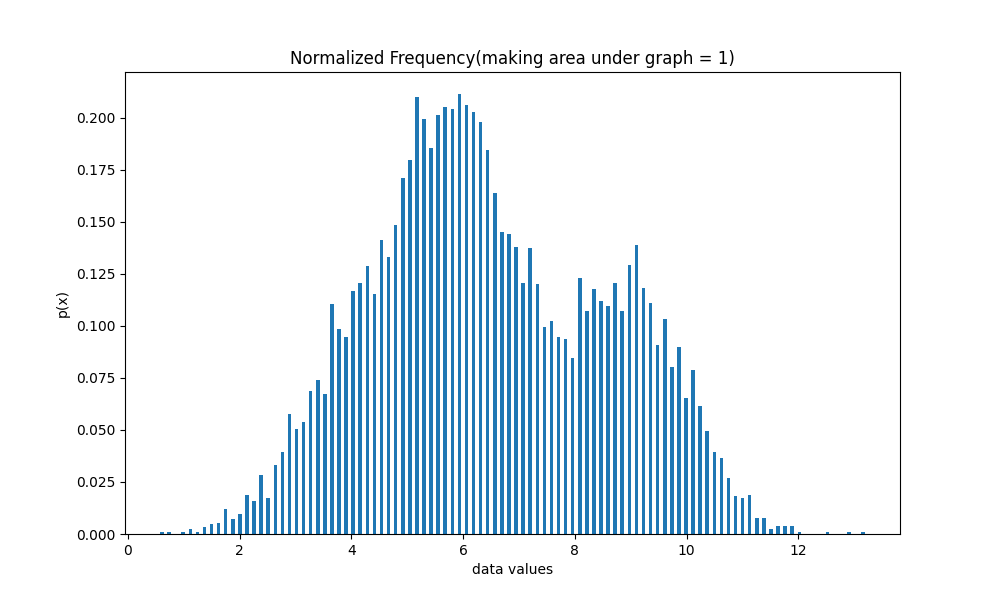
\includegraphics[width=0.5\textwidth]{images/3b.png}
        \captionof{figure}{Histogram }
    \end{center}
\end{minipage}
\subsection{Task C}
\textbf{\underline{Solution:}}\\
\\
\textbf{Check the code in 3.ipynb}
\\
\textbf{\underline{Proof: }}
\\
For first two moments $\mu_1^{bin}$ and $\mu_2^{bin}$ :
\\
Given,
\begin{equation}
\begin{split}
    \mu_1 &= E[X] \\
    \mu_2 &= E[X^2]
\end{split}
\end{equation}
As we know that, for binomial distribution
\begin{equation}
\begin{split}
     E[X] &= E[\sum_{i=1}^{n}Y_i]\\
          &= \sum_{i=1}^{n}E[Y_i]\\
          &= \sum_{i=1}^{n}p\\
     \mu_1 = E[X] &= np
\end{split}
\end{equation}
Where, $X_i = \sum_{i=1}^{n}Y_i$ and $Y_i \sim Bern(p)$
\begin{equation}
\begin{split}
     E[X^2] &= Var[X] + (E[X])^2\\
          &= np(1-p) + (np)^2\\
          &= np - n{p}^2 + n^2p^2\\
     \mu_2 = E[X^2] &= np + n(n-1)p^2
\end{split}
\end{equation}
Where, Var[X] = np(1-p) (for normal binomial distribution) and E[X] = np
\subsection{Task D}
\textbf{\underline{Solution:}}\\
\\
\textbf{Check the code in 3.ipynb}
\\
\textbf{\underline{Proof: }}
\\
We know that for first two moments $\mu_1^{Gamma} = E[X]$ and $\mu_2^{Gamma} = E[X^2]$ :
\begin{equation}
\begin{split}
    E[X] &= \int_{-\infty}^{\infty}xf_X(x)dx\\
         &= \int_{0}^{\infty}x(\frac{1}{\theta^k\tau(k)}x^{k-1}e^-\frac{x}{\theta})dx\\
         &= \frac{1}{\theta^k\tau(k)}\int_{0}^{\infty}x^{(k+1)-1}e^-\frac{x}{\theta}dx\\ 
         &= \frac{1}{\theta^k\tau(k)}(\theta^{k+1}\tau(k+1))\\
          &= \frac{\theta^{k+1}(k\tau(k))}{\theta^k\tau(k)}\\
         \mu_1 = E[X] &= k\theta
\end{split}
\end{equation}
Where we used some Gamma distribution properties like $\tau(k+1) = k\tau(k)$
\begin{equation}
\begin{split}
    E[X^2] &= \int_{-\infty}^{\infty}x^2f_X(x)dx\\
         &= \int_{0}^{\infty}x^2(\frac{1}{\theta^k\tau(k)}x^{k-1}e^-\frac{x}{\theta})dx\\
         &= \frac{1}{\theta^k\tau(k)}\int_{0}^{\infty}x^{(k+2)-1}e^-\frac{x}{\theta}dx\\ 
         &= \frac{1}{\theta^k\tau(k)}(\theta^{k+2}\tau(k+2))\\
          &= \frac{\theta^{k+2}(k(k+1)\tau(k))}{\theta^k\tau(k)}\\
         \mu_2 = E[X^2] &= k(k+1)\theta^2
\end{split}
\end{equation}
\subsection{Task E}
\textbf{\underline{Solution:}}\\
\\
\textbf{Check the code in 3.ipynb}
\subsection{Task F}
\textbf{\underline{Solution:}}\\
\\
\textbf{Check the code in 3.ipynb}
\section{Quality in Inequalities}
Given, Markov's Inequality
\begin{equation}
    P[X \geq a] \leq \frac{E[X]}{a}
\end{equation}
Where, 
    $X \geq 0, a>0$
\subsection{Task A}
\textbf{\underline{Solution:}}\\
\\
\textbf{Intuitive proof :}\\
    Let's assume that we have  boxes containing balls and the average number of balls per box is 10. The probability of finding more than 'a' balls in a box is P[X$\geq$a]. When a$\leq$10, $\frac{E[X]}{a}$ will be greater than 1 so markov's inequality holds. when a>10, as a goes further away from mean, P[X$\geq$a] keep decreasing. So, intuitively we can say that markov's inequality holds. \\
\\
\textbf{Rigorous proof :}\\
Let X be discrete Random Variables in ascending order and $x_m$= a 
To get $P[X\geq a]$, we can do as follows
\begin{equation}
\begin{split}
    E[X]& = \sum_{i=1}^{n}x_iP[x_i]dx \\
    & \geq \sum_{i=m}^{n}x_iP[x_i]dx \\
    & \geq \sum_{i=m}^{n}aP[x_i]dx \\
    & \geq a\sum_{i=m}^{n}P[x_i]dx \\
    E[X]& \geq aP[X\geq a]
\end{split}
\end{equation}

Therefore, we get
\begin{equation}
    P[X \geq a] \leq \frac{E[X]}{a}
\end{equation}
We can do similarly for continuous Random variables by limiting n to infinity.

\subsection{Task B}
\textbf{To be proved :}
\begin{equation}
    P[X-\mu \geq \tau] \leq \frac{\sigma^2}{\sigma^2+\tau^2} \forall \tau > 0
\end{equation}
Where, $\mu$ = mean of R.V, $\sigma$ = standard deviance of R.V \\
\\
\textbf{\underline{Solution:}}\\
We can write the following
\begin{equation}
\begin{split}
    P[X-\mu \geq \tau]& = P[X-\mu+\alpha \geq \tau+\alpha] \\
    & \leq P[(X-\mu+\alpha)^2 \geq (\tau+\alpha)^2] \\
\end{split}
\end{equation}
Where, $\alpha \geq -\tau$

we can apply the Markov's inequality to (2)
\begin{equation}
\begin{split}
    P[(X-\mu+\alpha)^2 \geq (\tau+\alpha)^2]& \leq \frac{E((X-\mu+\alpha)^2)}{(\tau+\alpha)^2} \\
    & \leq \frac{E((X-\mu)^2+2(X-\mu)\alpha+\alpha^2}{(\tau+\alpha)^2} \\
    & \leq \frac{E((X-\mu)^2)+2E((X-\mu))\alpha+\alpha^2}{(\tau+\alpha)^2} \\
\end{split}
\end{equation}
\begin{equation}
\begin{split}
    P[(X-\mu+\alpha)^2 \geq (\tau+\alpha)^2]& \leq \frac{\sigma^2+\alpha^2}{(\tau+\alpha)^2}
\end{split}
\end{equation}

\begin{equation}
\begin{split}
    P[X-\mu \geq \tau]& \leq \frac{\sigma^2+\alpha^2}{(\tau+\alpha)^2}
\end{split}
\end{equation}
We can further decrease the range in (5) by differentiating with $\alpha$. So that we get minimum value in right term.
\begin{equation}
\begin{split}
    \frac{d(\frac{\sigma^2+\alpha^2}{(\tau+\alpha)^2})}{d\alpha}& = 0 \\
    \frac{2\alpha(\tau+\alpha)-2(\sigma^2+\alpha^2)}{(\tau+\alpha)^3}& = 0 \\
    2\alpha(\tau+\alpha)& = 2(\sigma^2+\alpha^2) \\
    \alpha& = \frac{\sigma^2}{\tau}
\end{split}
\end{equation}

By substituting (6), we will get
\begin{equation}
    (\frac{\sigma^2+\alpha^2}{(\tau+\alpha)^2})_{min} = \frac{\sigma^2}{\sigma^2+\tau^2}
\end{equation}

So, from (7) and (5), we can conclude that
\begin{equation}
    P[X-\mu \geq \tau] \leq \frac{\sigma^2}{\sigma^2+\tau^2}
\end{equation}

\subsection{Task C}
\textbf{To be proved :}
\begin{equation}
    P[X\geq x] \leq e^{-xt}M_X(t) \forall t>0
\end{equation}
\begin{equation}
    P[X\leq x] \leq e^{-xt}M_X(t) \forall t<0
\end{equation}
\textbf{\underline{Solution:}}\\
We can write MGF for X as
\begin{equation}
    M_X(t) = \int_0^\infty e^{ty}P[X=y]dy 
\end{equation}

\begin{itemize}
    \item \underline{\textbf{Case 1 :}} t$>$0

Similar to the Method used in Task A, we can extend it to continuous and do the following
\begin{equation}
\begin{split}
    \int_0^\infty e^{ty}P[X=y]dy& \geq \int_x^\infty e^{ty}P[X=y]dy \\
    \int_0^\infty e^{ty}P[X=y]dy& \geq e^{tx}\int_x^\infty P[X=y]dy \\
    M_X(t)& \geq e^{tx}\int_x^\infty P[X=y]dy \\
    e^{-tx}M_X(t)& \geq \int_x^\infty P[X=y]dy \\
    e^{-tx}M_X(t)& \geq P[X\geq x]
\end{split}
\end{equation}
Hence, proved.
    \item \underline{\textbf{Case 2 :}} t$<$0

Similarly,
\begin{equation}
\begin{split}
    \int_0^\infty e^{ty}P[X=y]dy& \geq \int_0^x e^{ty}P[X=y]dy \\
    \int_0^\infty e^{ty}P[X=y]dy& \geq e^{tx}\int_0^x P[X=y]dy \\
    M_X(t)& \geq e^{tx}\int_0^x P[X=y]dy \\
    e^{-tx}M_X(t)& \geq \int_0^x P[X=y]dy \\
    e^{-tx}M_X(t)& \geq P[X\geq x]
\end{split}
\end{equation}
Hence, proved.
\end{itemize}

\subsection{Task D}
\textbf{\underline{Solution:}} \\
For, n i.i.ds, $X_1, X_2, \dots, X_n$, which have Bernouli distribution with E[$X_i$]$=$ $p_i$, Y can be written as $Y=\sum_{i=1}^nX_i$\\
\begin{enumerate}
    \item \textbf{Expectation of Y}

As all X's are independent and identically distributed, we can do as follows
\begin{equation}
\begin{split}
    E[Y]& = E[X_1+ X_2+ \dots+ X_n] \\
    & = E[X_1]+E[X_2]+\dots+E[X_n] \\
    & = \sum_{i=1}^np_i \\
    & = np_i
\end{split}
\end{equation}
\\
    \item \textbf{Prove:}

\begin{equation}
    P[Y \geq (1+\delta)\mu] \leq \frac{e^{\mu(e^t-1)}}{e^{(1+\delta)t\mu}}
\end{equation}
Where, $\mu$ = expectation of Y, $\delta>-1, t>0$ \\
\\
Using (1) of Task C, we can write that
\begin{equation}
\begin{split}
    P[Y \geq (1+\delta)\mu]& \leq e^{-t(1+\delta)\mu}M_Y(t), t>0 \\
    & \leq e^{-t(1+\delta)\mu}E[e^{Yt}] \\
    & \leq e^{-t(1+\delta)\mu}E[e^{t\sum_{i=1}^nX_i}]\\
\end{split}
\end{equation}

As X's are i.i.d, we can write
\begin{equation}
\begin{split}
     P[Y \geq (1+\delta)\mu]& \leq e^{-t(1+\delta)\mu}\prod_{i=1}^nE[e^{tX_i}] \\
     P[Y \geq (1+\delta)\mu]& \leq e^{-t(1+\delta)\mu}\prod_{i=1}^n(1+p_i(e^t-1)) \\
     P[Y \geq (1+\delta)\mu]& \leq e^{-t(1+\delta)\mu}(1+p_i(e^t-1))^n \\
\end{split}
\end{equation}

Now using the inequality $1+a < e^a, \forall a>0$, we can write
\begin{equation}
\begin{split}
    e^{-t(1+\delta)\mu}(1+p_i(e^t-1))^n& \leq e^{-t(1+\delta)\mu}e^{p_i(e^t-1)n} \\
    e^{-t(1+\delta)\mu}(1+p_i(e^t-1))^n& \leq e^{-t(1+\delta)\mu}e^{\mu(e^t-1)} \\
    P[Y \geq (1+\delta)\mu]& \leq e^{-t(1+\delta)\mu}e^{\mu(e^t-1)} \\
\end{split}
\end{equation}

Therefore, we can conclude that
\begin{equation}
    P[Y \geq (1+\delta)\mu] \leq \frac{e^{\mu(e^t-1)}}{e^{(1+\delta)t\mu}}
\end{equation}

    \item \textbf{Improve the bound with appropriate t}

Using (2), to improve bound, we need to minimise right term. We can do so by differentiating right term with t and equating it with 0.
\begin{equation}
\begin{split}
    \frac{d(\frac{e^{\mu(e^t-1)}}{e^{(1+\delta)t\mu}})}{dt}& = 0 \\
    \mu(e^t) - (1+\delta)\mu& = 0 \\
    e^t& = 1 + \delta \\
\end{split}
\end{equation}

From (3), we get t = ln($1+\delta$). By substituting it in (2), we get
\begin{equation}
\begin{split}
    P[Y \geq (1+\delta)\mu]& \leq \frac{e^{\mu\delta}}{(1+\delta)^{(1+\delta)\mu}} \\
    \frac{e^{\mu\delta}}{(1+\delta)^{(1+\delta)\mu}}& = e^{\mu\delta-(1+\delta)ln(1+\delta)\mu} \\
\end{split}
\end{equation}
\begin{itemize}
    \item \textbf{Case 1:}  $\delta > 0$

We can use $ln(1+\delta) \geq \frac{2\delta}{2+\delta}$ and get:
\begin{equation}
\begin{split}
      e^{\mu\delta-(1+\delta)ln(1+\delta)\mu}& \leq e^{\mu\delta-(1+\delta)\frac{2\delta}{2+\delta}\mu}
\end{split}
\end{equation}
Therefore,
\begin{equation}
    P[Y \geq (1+\delta)\mu] \leq e^{-\frac{\mu\delta^2}{2+\delta}}
\end{equation}
    \item \textbf{Case 2:}  $-1 < \delta < 0 $

Similarly, we can use $ln(1+\delta) \geq \frac{\delta(\delta+2)}{2(\delta+1)}$ and get:
\begin{equation}
\begin{split}
      e^{\mu\delta-(1+\delta)ln(1+\delta)\mu}& \leq e^{\mu\delta-(1+\delta)\frac{\delta(\delta+2)}{2(\delta+1)}}
\end{split}
\end{equation}

Therefore,
\begin{equation}
    P[Y \leq (1+\delta)\mu] \leq e^{-\frac{\mu\delta^2}{2}}
\end{equation}
\end{itemize}
\end{enumerate}
\subsection{Task E} 
\textbf{\underline{Solution:}}\\
\textbf{To be Proved:}\\
Let $X_1,X_2,\dots,X_n$ be i.i.d random variables with each having mean $ \mu $.We define $ A_n = \frac{\sum_{i=1}^nX_i}{n} $. Then for all $ \epsilon > 0 $,we have
\begin{equation}
    \lim_{n\to\infty}P[|A_n - \mu| > \epsilon] = 0
\end{equation}
First lets remove modulus and bound it to the minimum range(just like chernoff's bound)
\begin{equation}
    P[|A_n - \mu| > \epsilon] = P[A_n - \mu > \epsilon] + P[A_n - \mu < -\epsilon]
\end{equation}
Lets first assume the sum $ S_n = \sum_{i=1}^{n}X_i$, so $A_n = \frac{S_n}{n}$
\begin{itemize}
    \item First lets focus on $P[A_n > \mu + \epsilon]$
\begin{equation}
    P[A_n > \mu+\epsilon]=P[S_n > n(\mu+\epsilon)] \leq e^{-tn(\mu+\epsilon)}E[tS_n]
\end{equation}
Since $X_1,X_2,\dots,X_n$ are independent , the M.G.F of $S_n$ is a product of M.G.Fs of $X_i's$
\begin{equation}
\begin{split}
    E[e^{tS_n}] &= (E[e^{tX_i}]^n\\
    P(S_n > n(\mu+\epsilon) &\leq ( e^{-t(\mu+\epsilon)}E[e^{tX_i}])^n
\end{split}
\end{equation}
To get the minimum range in the bound,we need to minimize the R.H.S W.R.T t.\\

$f(t) = e^{-t(\mu+\epsilon)}E[e^{tX_i}]$\\

Here we don't need the exact value of t because the limits we are applying are on 'n' whereas the function f(t) doesnt depend on n, we just need to know that for some choice of t:
\begin{equation}
     P(S_n > n(\mu+\epsilon) \leq e^{-cn}
\end{equation}
Where, c is a constant W.R.T n.\\
\item Similarly for $P[A_n - \mu < -\epsilon]$:
\begin{equation}
\begin{split}
     P[A_n  < \mu -\epsilon] &= P[S_n < n( \mu -\epsilon)]\\
     P[S_n < n( \mu -\epsilon)] &\leq e^{-cn} 
\end{split}
\end{equation}
\end{itemize}
Now by combining the bounds:
\begin{equation}
    P[|A_n - \mu| > \epsilon] \leq (e^{-cn} + e^{-cn} = 2e^{-cn}) 
\end{equation}
Now applying $\lim_{n\to\infty}$ on B.S:
\begin{equation}
    \lim_{n\to\infty}P[|A_n - \mu| > \epsilon] \leq \lim_{n\to\infty}2e^{-cn}
\end{equation}
As $n \to \infty$ , $\lim_{n\to\infty}2e^{-cn} \to 0$ and we know that
$P[|A_n - \mu| > \epsilon] \geq 0$\\
Therefore:
\begin{equation}
     \lim_{n\to\infty}P[|A_n - \mu| > \epsilon] = 0
\end{equation}
\section{A Pretty "Normal" Mixture}
\subsection{Task A}
\textbf{\underline{Solution:}}

\subsection{Task B}
\textbf{\underline{Solution:}}
\begin{enumerate}
    \item \textbf{E[X]}
    
As X is GMM sampled, we can write it’s expectation as
\begin{equation}
    E[X] = \sum_{i=1}^{k} p_iE[X_i]
\end{equation}
Also, we know that 

\begin{equation}
    E[X_i] = \mu_i
\end{equation}
From (1) and (2),

\begin{equation}
   \mu = E[X] = \sum_{i=1}^{k} p_i\mu_i
\end{equation}
    \item \textbf{Var[X]}

For a GMM, acc to Law of Total Variance, Var[X] can be written as
\begin{equation}
\begin{split}
    Var[X]& = E[Var[X_i]] + Var[E[X_i]] \\
    & = \sum_{i=1}^{k} p_iVar[X_i] + Var[\sum_{i=1}^{k} p_i\mu_1|\mu]
\end{split}
\end{equation}

For the second term, 
\begin{equation}
    Var[\sum_{i=1}^{k} p_i\mu_i|\mu] = \sum_{i=1}^{k}p_i(\mu_i - \mu)^2
\end{equation}

From (4) and (5),
\begin{equation}
    Var[X] = \sum_{i=1}^{k} p_i\sigma_i^2 + \sum_{i=1}^{k}p_i(\mu_i - \mu)^2
\end{equation}

    \item \textbf{The MGF, M(t) of X}

MGF of a GMM is
\begin{equation}
    M_X(t) = \sum_{i=1}^{k} p_iM_X_i(t)
\end{equation}
For a Normal Guassian variable,
\begin{equation}
\begin{split}
    M_X_i(t)& = E[e^{tX_i}] \\
    & = \int_{-\infty}^{\infty} e^{tx} \frac{1}{\sqrt{2\pi}\sigma_i}e^{\frac{-(x-\mu_i)^2}{2\sigma_i^2}}dx \\
    & = e^{t\mu_i + \frac{1}{2}t^2\sigma_i^2}\frac{1}{\sqrt{2\pi}\sigma_i} \int_{-\infty}^{\infty} e^{-\frac{(x-(\mu_i+\sigma_i^2t))^2}{2\sigma_i^2}}dx \\
    M_X_i(t)& = e^{t\mu_i + \frac{1}{2}t^2\sigma_i^2}
\end{split}
\end{equation} 

From (7) and (8),
\begin{equation}
    M_X(t) = \sum_{i=1}^k p_ie^{t\mu_i + \frac{1}{2}t^2\sigma_i^2}
\end{equation}
\end{enumerate}

\subsection{Task C}
\textbf{\underline{Solution:}}
Given random variable Z as
\begin{equation}
    Z = \sum_{i=1}^kp_iX_i
\end{equation}
\begin{enumerate}
    \item \textbf{E[Z]}

We can write expectation of Z similar to the GMM above.
\begin{equation}
\begin{split}
    E[Z]& = E[\sum_{i=1}^kp_iX_i] \\
    & = \sum_{i=1}^kp_iE[X_i]
\end{split}
\end{equation}

Therefore,
\begin{equation}
    E[Z] = \sum_{i=1}^kp_i\mu_i
\end{equation}

    \item \textbf{Var[Z]}

acc to the formula for variance calculation of sum of independent random variables
\begin{equation}
\begin{split}
    Var[Z]& = p_1^2Var[X_1]+p_2^2Var[X_2]+\dot+p_k^2Var[X_k] \\
    & = \sum_{i=1}^k p_i^2\sigma^2_i
\end{split}
\end{equation}



    \item \textbf{The PDF, $\textit{f}_Z(u)$, of Z}

As Z is a Normal Gaussian Distribution which we can say by comparing MGF, PDF of Z is
\begin{equation}
    \textit{f}_Z(u) = \frac{1}{\sqrt{2\pi}\sigma}e^{-\frac{(u-\mu)^2}{2\sigma^2}}
\end{equation}
\begin{center}
    Where,  
          $\mu = \sum_{i=1}^kp_i\mu_i,   \sigma^2 = \sum_{i=1}^kp_i^2\sigma^2_i$
\end{center}

    \item \textbf{The MGF, $M_Z(t)$, of Z}

For MGF,
\begin{equation}
    \begin{split}
        M_Z(t)& = E(e^{Zt}) \\
        & = E(e^{(p_1X_1+p_1X_2+\dots+p_kX_k)t}) \\
        & = E(e^{p_1X_1t})E(e^{p_2X_2t})\dots E(e^{p_2X_kt}) \\
        & = \prod_{i=1}^k e^{tp_i\mu_i+\frac{1}{2}p_i^2\sigma^2_it^2} \\
        & = e^{t\sum_{i=1}^kp_i\mu_i + \frac{1}{2}t^2\sum_{i=1}^kp_i^2\sigma^2_i} \\
    \end{split}
\end{equation}
\begin{equation}
    M_Z(t) = e^{t\mu+t^2\frac{1}{2}\sigma^2}
\end{equation}
\begin{center}
    Where,  
          $\mu = \sum_{i=1}^kp_i\mu_i,   \sigma^2 = \sum_{i=1}^kp_i^2\sigma^2_i$
\end{center}

Here, MGF is similar to Normal Gaussian randam variables.
    \item \textbf{Conclusion}

Weighted sum of Normal Gaussian variables, Z, is different from GMM, X. They have same expectation but remaining properties are different.

Therefore, we can conclude that Z and X have different properties.

    \item \textbf{Type of Distribution}

Z follows Normal Gaussian Distribution.
\end{enumerate}

\subsection{Task D}
\textbf{\underline{Solution:}}\\
For a finite discrete random variable X,we need to show that  its MGF and PDF uniquely determine each other.\\
To do so, we need to complete proving 2 parts,i.e., given a PDF, there exist a unique MGF and vice-versa.\\
\\
Let's take a finite discrete random variable X with PDF, P[X=$x_i$] = $p_i$, and MGF, $M_X$(t) = $\sum_{i=1}^ne^{x_it}p_i$.\\
\\
\textbf{\underline{Proof of uniqueness :}}
\\
\begin{enumerate}
    \item \textbf{PDF to MGF :}\\
\\
It is simpler to prove this direction. 
\begin{itemize}
    \item For a given PDF P, we can always write MGF,$M_X$(t), as $\sum_{i=1}^ne^{x_it}p_i$.
    \item The MGF can be uniquely defined for a particular X and its corresponding PDF,P.
\end{itemize}

    \item \textbf{MGF to PDF :}\\
\\
Now let's take two random variables X, Y with $M_X(t)$ = $M_Y(t)$.
\begin{itemize}
    \item We can write $M_X(t)$ as $\sum_{i=1}^ne^{x_it}p(x_i)$ and $M_Y(t)$ as $\sum_{i=1}^ne^{y_it}p(y_i)$.
    \item Using Taylor series we can split them into powers of t as follows:
\begin{equation}
    M_X(t) = \sum_{i=1}^n(\sum_{k=0}^\infty \frac{t^kx_i^k}{k!})p(x_i)
\end{equation}
\begin{equation}
    M_Y(t) = \sum_{i=1}^n(\sum_{k=0}^\infty \frac{t^ky_i^k}{k!})p(y_i)
\end{equation}
    \item As we already assumed $M_X(t)$ = $M_Y(t)$, we get 
\begin{equation}
    \sum_{i=1}^n(\sum_{k=0}^\infty \frac{t^kx_i^k}{k!})p(x_i) = \sum_{i=1}^n(\sum_{k=0}^\infty \frac{t^ky_i^k}{k!})p(y_i)
\end{equation}
    \item By comparing $t^k$ coefficients, we get
\begin{equation}
    \sum_{i=1}^n\frac{x_i^k}{k!}p(x_i) = \sum_{i=1}^n\frac{y_i^k}{k!}p(y_i) ,\forall k\in W
\end{equation}
    \item As the given equation satisfy for all k, from the properties of linear equations with p($x_i$) and p($y_i$) as unknowns, equation has unique solutions.
    \item  Hence, we can say that there is unique PDF for a given MGF.
\end{itemize}
From 1 and 2, we can conclude that for a finite discrete random variable X,its MGF and PDF uniquely determine each other.\\
\textbf{Conclusion for X and Z:}
\\
\begin{itemize}
    \item Z is a simple Gaussian because its MGF corresponds to that of a normal distribution,confirming it has a unique Gaussian PDF.
    \item X is not Gaussian even though its MGF uniquely determines its distribution.X's distribution is a more complex mixture of Gaussians which depends on the probability selection of different Gaussian components.
\end{itemize}
\end{enumerate}
\end{document}
